% Copertina (riproduzione della copertina originale)
\newgeometry{margin=0pt}
\definecolor{verdecopertina}{RGB}{50,163,124}
\pagecolor{verdecopertina}
\begin{titlepage}
\color{white}\fontfamily{ptm}\selectfont
\noindent\begin{picture}(0,0)
\put(10.5cm,-2.03cm){\makebox[0pt]{\fontsize{30}{30}\selectfont\bfseries Luigi E. Picasso}}
\put(10.5cm,-5.93cm){\makebox[0pt]{\fontsize{56}{56}\selectfont Lezioni}}
\put(10.5cm,-7.63cm){\makebox[0pt]{\fontsize{56}{56}\selectfont di}}
\put(10.5cm,-9.23cm){\makebox[0pt]{\fontsize{56}{56}\selectfont Fisica Generale 2}}
\put(10.5cm,-19.63cm){\makebox[0pt]{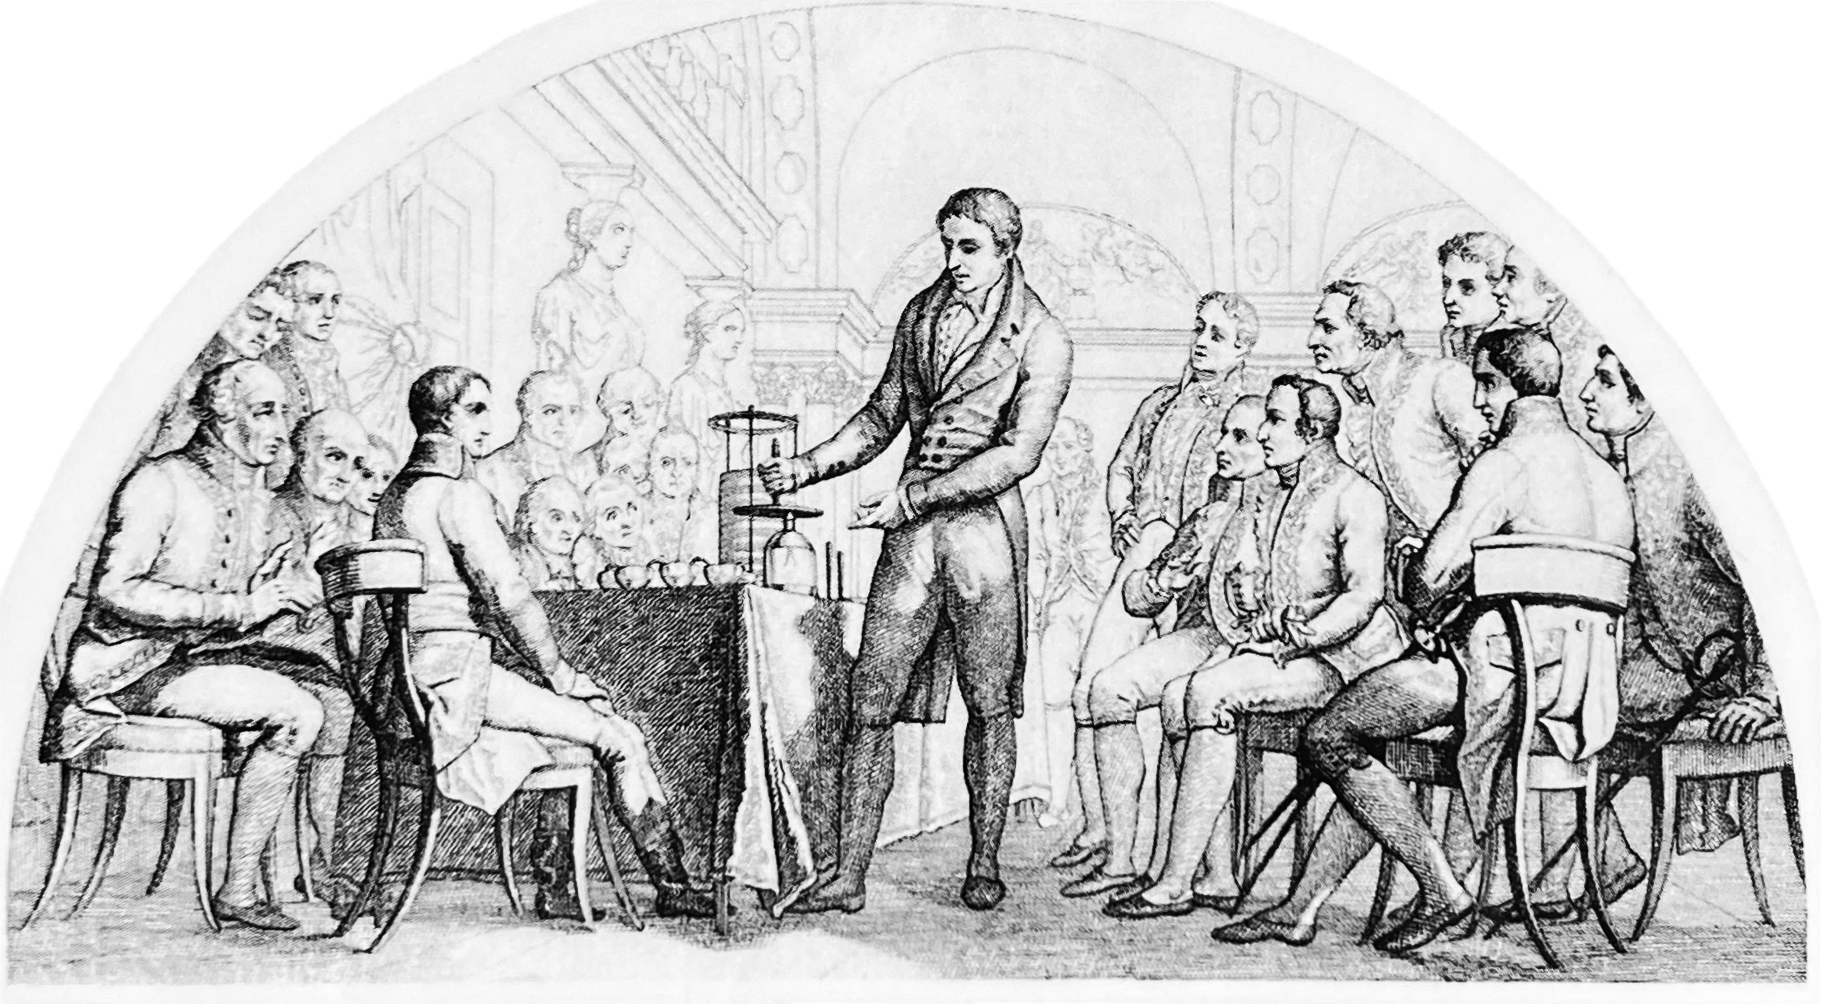
\includegraphics[width=15.1cm]{fig/cover}}}
\put(10.5cm,-27.49cm){\makebox[0pt]{\fontsize{13}{13}\selectfont\bfseries EDIZIONI ETS}}
\end{picture}
\end{titlepage}
\nopagecolor
\restoregeometry
